\chapter{Anexo I: Árbol del problema}

\begin{figure}[h]
		\begin{center}
			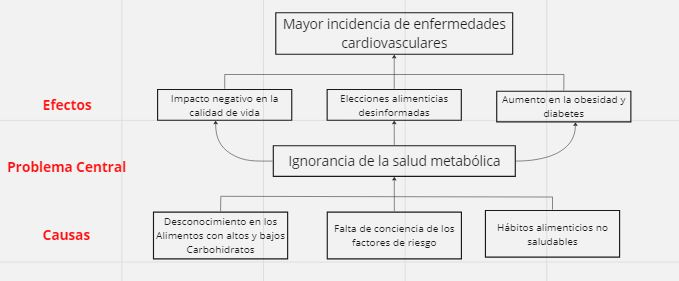
\includegraphics[width=1.1\textwidth]{1/figures/arbol de problems.JPG}
			\caption{Prueba de Figura}
			\label{fig1}
		\end{center}
		
	\end{figure}

\chapter{Anexo II: Árbol del objetivos}

\begin{figure}[h]
		\begin{center}
			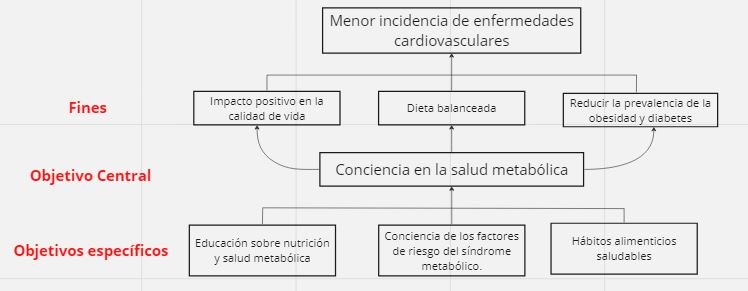
\includegraphics[width=1.1\textwidth]{1/figures/arbol de objetivos.JPG}
			\caption{Prueba de Figura}
			\label{fig1}
		\end{center}
		
	\end{figure}

\chapter{Anexo III: Matriz de Consistencia}

\begin{table}[h!]
	\centering
	\small
	\begin{tabular}{ |m{5cm}|m{5cm}|m{5cm}| }
		\hline
		\rowcolor{bluejean}
		\Centering \color{white}{PROBLEMAS}& \Centering \color{white}{OBJETIVOS}& \Centering \color{white}{HIPÓTESIS}\\
		\hline
		\rowcolor{turq}
		\Centering Problema General& \Centering Objetivo General & \Centering Hipotesis General \\
		\hline
  
        \ProblemaGeneral & 
        \ObjetivoGeneral  & 
        \HipotesisGeneral \\
        \hline
		
        \rowcolor{turq}
		\Centering Problemas Específicos& \Centering Objetivos Específicos & \Centering Hipotesis Específicas \\
		\hline
  
		{\Pbone} & {\Objone} & {\Hone} \\
		\hline
		{\Pbtwo} & {\Objtwo} & {\Htwo} \\
		\hline
		{\Pbthree} & {\Objthree} & {\Hthree} \\
		\hline
            {\Pbfour} & {\Objfour} & {\Hfour} \\
		\hline
	\end{tabular}
	\caption{Matriz de consistencia. Fuente: Elaboración propia}
	\label{1:table}
\end{table}






